\section{The LMC and inherited gravitating stock}
\label{sec:lmc}

For $3\times10^9\Msun$ of LMC baryons, the retained-stock prescription gives
\begin{equation}
M(<30\,\mathrm{kpc})=5.0348\times10^{10}\Msun,
\qquad
M(<50\,\mathrm{kpc})=8.2896\times10^{10}\Msun.
\label{eq:lmcmasses}
\end{equation}
Warren et al. infer $(4.7$--$5.1)\times10^{10}\Msun$ inside 30 kpc from
the Orphan--Chenab stream. Brooks et al. infer
$8.76^{+1.94}_{-1.77}\times10^{10}\Msun$ inside 50 kpc from outer-halo
kinematics. The calculated masses agree with both quoted results.
\cite{warren,brooks}

In the same baryonic configuration, the tested QUMOND external-field
calculations give only $(1.54$--$1.68)\times10^{10}\Msun$ of effective
enclosed LMC mass inside 30 kpc. The difference comes from whether the
system retains its previously established stock when it enters the Milky
Way environment. \source{G1, G2}

\subsection{From an acceleration law to an enclosed mass}

Outside most of the LMC's baryons, use the spherical point-source
approximation
\begin{equation}
g_b(r)=\frac{GM_b}{r^2},\qquad
r_M=\sqrt{\frac{GM_b}{a_0}}.
\end{equation}
Equation~\eqref{eq:rar} then gives
\begin{equation}
g_{\rm obs}(r)=\frac{GM_b}{r^2[1-e^{-r_M/r}]}.
\end{equation}
The effective enclosed mass is defined through $g_{\rm obs}=GM(<r)/r^2$,
so
\begin{equation}
M(<r)=\frac{M_b}{1-e^{-r_M/r}},\qquad
M_R(<r)=M(<r)-M_b.
\label{eq:lmcprofile}
\end{equation}
The baryonic term and the extra stock are counted once each.

With $G=4.30091\times10^{-6}\,\mathrm{kpc}\,(\mathrm{km/s})^2\Msun^{-1}$,
$a_0=3798.47\,(\mathrm{km/s})^2\mathrm{kpc}^{-1}$, and the stated baryonic
mass, $r_M=1.84305\,\mathrm{kpc}$. At 30 kpc the exponent is
$r_M/r=0.061435$, and
\begin{equation}
M(<30)=\frac{3\times10^9}{1-e^{-0.061435}}\Msun
=5.0348\times10^{10}\Msun.
\end{equation}
At 50 kpc the exponent is $0.036861$, giving the second mass in
equation~\eqref{eq:lmcmasses}. A Plummer baryonic profile with scale
$1.5\,\mathrm{kpc}$ changes these outer values only slightly.

In the deep regime,
\begin{equation}
M(<r)=\sqrt{\frac{M_ba_0}{G}}\,r+\frac{M_b}{2}
+O(r_M/r).
\end{equation}
The enclosed mass grows approximately linearly with radius, giving an
approximately flat circular speed before the finite stock budget limits
the profile. This also shows the main sensitivity:
$M(<r)\propto M_b^{1/2}a_0^{1/2}r$. A fractional baryonic-mass error
contributes about half as much fractional mass error at these radii.
The central numbers do not imply negligible uncertainty in the baryons.

\subsection{Why the budget refers to ancestral baryons}

The initial commitment is bounded by $M_{b,L}/\epsilon$, where $M_{b,L}$
is the baryonic content of the Lagrangian source whose history is followed.
In the linear-depletion benchmark used for the saved galaxy calculations,
a full release removes the share $\eta_*$. Its carrier budget is
\begin{equation}
M_R\le \frac{1-\eta_*}{\epsilon}M_{b,L},\qquad
C_R\equiv\frac{M_{R,\max}}{M_{b,\rm present}}.
\label{eq:cap}
\end{equation}
Loss of gas or redistribution of baryons can make $C_R$ much larger than
$1/\epsilon$. A large present stock-to-star ratio is compatible with a
finite initial commitment per ancestral baryon.

Writing $M_{b,L}=f_bM_h$ gives the manuscript's useful parameterization
\begin{equation}
C_R\simeq(1-\eta_*)(1-f_b)\frac{M_h}{M_{b,\rm present}},
\end{equation}
when $f_b/(1-f_b)\simeq\epsilon$. Here $M_h$ identifies the ancestral
assembly mass used for the budget. It is an astrophysical history input.
Its use does not follow from the cell count alone.

The numerical LMC model uses $C_R=33$, so the total mass cap is
$(1+C_R)M_b=1.02\times10^{11}\Msun$. Equation~\eqref{eq:lmcprofile} reaches
that cap at
\begin{equation}
r_{\rm cap}=-\frac{r_M}{\ln[1-(1+C_R)^{-1}]}=61.74\,\mathrm{kpc}.
\end{equation}
The quoted 30 and 50 kpc predictions lie inside the cap. Their values
are insensitive to its exact location. The composition-preserving
allocation replaces $1-\eta_*$ by $e^{-\eta_*}$ for complete ensemble
release, increasing this budget by $0.0455\%$. The reported masses and
satellite trajectories retain their original benchmark convention. \source{T1, O.3; G1}

\subsection{Persistence, transport, and tidal stripping}

Retained stock has a positive density and an advected mass. A collisionless
description uses a phase-space distribution $f_R(\mathbf x,\mathbf v,t)$
obeying
\begin{equation}
\frac{\partial f_R}{\partial t}
+\mathbf v\cdot\nabla_x f_R
-\nabla\Phi\cdot\nabla_v f_R=0,
\qquad
\rho_R=\int f_R\,d^3v,
\label{eq:vlasov}
\end{equation}
between formation, release, and carrier-reorganization events. Integrating
over velocity gives a continuity equation for $\rho_R$. A change in the
host's gravitational field can move the stock, distort it, or remove some
of it from the satellite. It does not algebraically erase its mass.

A spatially uniform external acceleration mainly accelerates the carrier
as a whole. Tides arise from the field gradient, represented locally by
$\partial_i\partial_j\Phi_{\rm host}$. They can unbind the extended stock
because its outer orbits are weakly bound. This is the physical difference
between losing stock through transport and reducing a static effective
gravity law because the external field changed.

The theory's equilibrium contact and its persistent-stock dynamics are
different stages of the same proposed mechanism. The contact specifies a
target profile for a coherent carrier; collisionless evolution follows
that profile after infall. The manuscript also allows mass-conserving
relaxation toward carrier-resolved equilibrium. The available satellite
runs use retained stock with no subsequent contact relaxation. Its rate
and its derivation from the native microscopic dynamics remain to be fixed.

\subsection{The external-field comparison}

In QUMOND, the field equation contains the nonlinear flux
$\nu(|\mathbf g_N|/a_0)\mathbf g_N$, where the Newtonian field includes
both host and satellite. The local calculation estimates the LMC's
equivalent enclosed mass by subtracting the host-only flux:
\begin{align}
M_{\rm LMC}^{Q}(<r)=-\frac1{4\pi G}\oint_{S_r}
\Big[&\nu\!\left(\frac{|\mathbf g_{N,L}+\mathbf g_{N,MW}|}{a_0}\right)
(\mathbf g_{N,L}+\mathbf g_{N,MW})\nonumber\\
&-\nu\!\left(\frac{|\mathbf g_{N,MW}|}{a_0}\right)
\mathbf g_{N,MW}\Big]\cdot d\mathbf A.
\label{eq:flux}
\end{align}
This is an effective gravitational mass, not a count of extra matter
particles. The host subtraction matters because the flux is nonlinear.

The computation uses a $10^{10}\Msun$ Hernquist bulge, a
$5\times10^{10}\Msun$ Miyamoto--Nagai disk, a $3\times10^9\Msun$
Plummer LMC, and a 50 kpc separation. Direct angular quadrature uses
96 Gauss--Legendre points and 192 azimuthal points. Re-execution gives
\begin{center}
\begin{tabular}{lc}
\toprule
Response prescription & $M(<30\,\mathrm{kpc})/[10^{10}\Msun]$\\
\midrule
Retained spherical stock & 5.035\\
QUMOND, exponential RAR function & 1.679\\
QUMOND, simple function & 1.681\\
QUMOND, standard function & 1.539\\
\bottomrule
\end{tabular}
\end{center}
The tested external-field models fall a factor of roughly three below the
cited 30 kpc inference. The difference persists across these three
interpolation choices. A complete comparison would evolve the observed
stream in each time-dependent model and compare its positions and
velocities directly. The published mass posterior was inferred using
gravitational models; it is not a raw model-free datum.

\begin{figure}[htbp]
\centering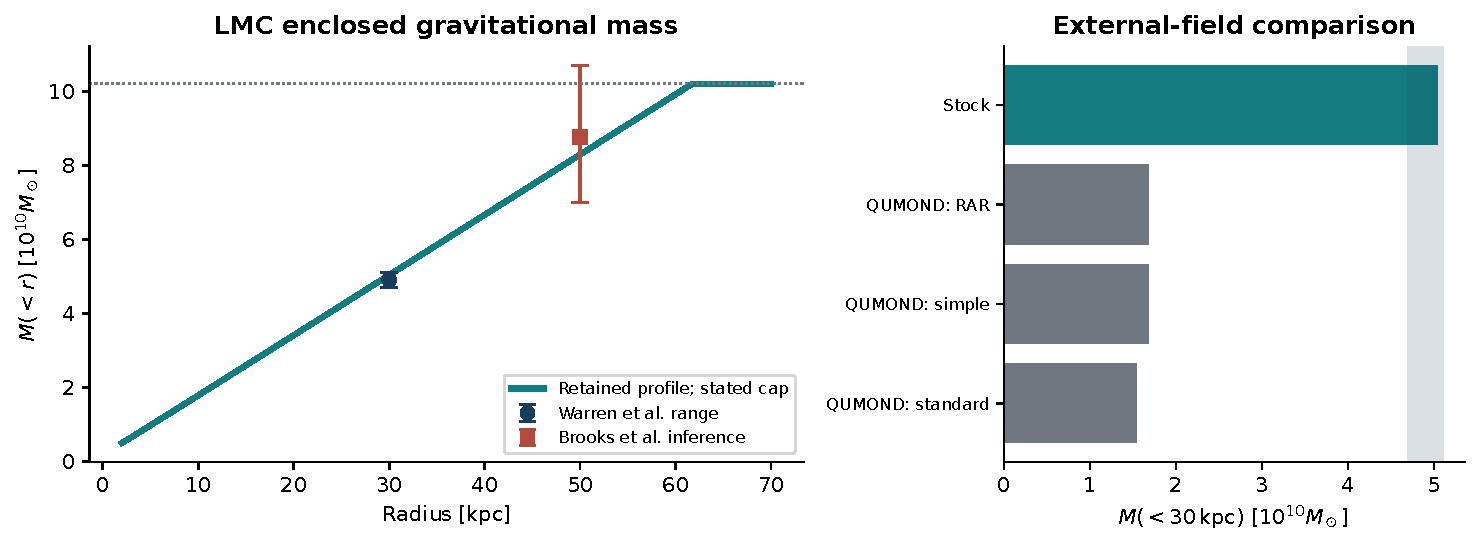
\includegraphics[width=\textwidth]{figures/lmc.pdf}
\caption{The retained LMC mass profile, its finite budget, and the
recomputed QUMOND flux comparison. The 30 kpc bar represents the reported
range of stream inferences, not a Gaussian one-sigma interval. The 50 kpc
bar uses the published asymmetric uncertainties.}
\end{figure}

\subsection{The reflex motion tests inertia}

An extended gravitating component should also accelerate the Milky Way.
Brooks et al. infer a reflex speed
$38.6^{+8.3}_{-7.8}\,\kms$ relative to halo stars at 100 kpc, jointly
with the LMC and Milky Way masses. That observable tests the dynamical
interaction, including the response of the outer halo. \cite{brooks}

The available moving-LMC calculation produces a Milky Way acceleration
corresponding to about $35\,\kms$ over the last gigayear. This establishes
the relevant scale. A direct comparison requires the same halo reference
population, spatial selection, and velocity estimator as the observation.
The present calculation also uses the usual asymmetric pair-force
approximation, while the theory requires reciprocal forces from its joint
source action. These distinctions prevent a precise reflex likelihood
claim from being assigned to the saved run. \source{G4}

The physical implication of a successful reflex calculation would be
strong: the extra gravity would participate in the momentum balance of
the system. Agreement of an isolated rotation curve alone cannot establish
that property.

\subsection{Tidal dwarfs test which source owns the response}

A tidal dwarf forms from material pulled out of a larger galaxy. Its gas
and stars already belong to an ancestral source. The carrier rule assigns
them to that inherited record while the parent remains dynamically
coherent. Applying a new isolated equilibrium law to the dwarf's own
baryons would count a new independent response at the wrong stage of its
history.

Exact projectors act on disjoint active record labels. Smooth spatial
weights used to distribute an effective source form a separate partition
of unity; they carry no projector-idempotence requirement. If $P$
is the active parent, its descendants contribute to the parent source
before the nonlinear response is evaluated. Parent and child are not
simultaneously counted as independent sources of an extra halo. A
descendant in the parent's retained response also inherits its director,
the orientation field that controls the transverse flux.
\source{T1, section 15 and N.8}

The director's stiffness controls its response to a local tilt of the
source. In the linearized description, a mode of wavenumber $k$ has
transfer factor
\begin{equation}
\frac{\delta\boldsymbol n(k)}{\delta\boldsymbol n_{\rm eq}(k)}
=\frac{1}{1+k^2\xi^2},
\end{equation}
where $\xi$ is the director coherence length fixed by the effective
stiffness. A descendant samples the parent's coherent director. A
separate carrier has its own stiffness and director. The inherited
orientation suppresses the local transverse response that the
independent-carrier calculation would allow. \source{G5}

The numerical proxy converts each resulting force field into a virial
dispersion. For a stationary tracer distribution of mass $M$, define
\begin{equation}
W=-\int\rho(\boldsymbol r)\,
\boldsymbol r\cdot\boldsymbol\nabla\Phi\,d^3r.
\end{equation}
The scalar virial relation $2K+W=0$ gives the direction-averaged
one-dimensional dispersion $\sigma^2=-W/(3M)$, and hence the boost
$\sigma^2/\sigma_N^2=W/W_N$. The force calculation, inherited orientation,
and tracer profile determine this ratio. The observed gas rotation still
requires a separate geometrical and dynamical interpretation.

The available NGC 5291 comparison uses three dynamical-to-baryonic mass
ratios, $1.5\pm0.7$, $1.3\pm0.5$, and $1.2\pm0.7$, and a parent of
$2\times10^{11}\Msun$ at 60 kpc. The inherited response gives modest
enhancements. Treating the dwarfs as separate isolated carriers gives
much larger enhancements. \source{G1, G5}\cite{lelli}
\begin{center}
\begin{tabular}{lcc}
\toprule
Prescription & Mass enhancement & Reported $\chi^2$ for three objects\\
\midrule
Parent-carrier inheritance & 1.5--2.0 & 0.5\\
Separate isolated carriers & 3.6--4.9 & 48\\
Newtonian baryons & 1.0 & 1.0\\
\bottomrule
\end{tabular}
\end{center}
The calculation uses a virial-response proxy, with the enhancement read
through $\sigma^2/\sigma_N^2$. It does not supply a resolved,
non-equilibrium gas-dynamical fit to every dwarf. Its evidential force is
the rejection of the separate-carrier prescription within this test.
Newtonian baryons also fit these ratios, so these three objects do not
uniquely select the capacity model or exclude conventional tidal dwarfs.
